\documentclass[10pt]{article}
\usepackage{float}
\usepackage{amsmath}
\usepackage{paralist}
\usepackage{setspace}
\usepackage{listings}
\usepackage{graphicx}
\usepackage[english]{babel}
\usepackage{geometry}
\usepackage{subcaption}
\usepackage[utf8]{inputenc}
\usepackage{listings}
\usepackage{color}
\usepackage{subcaption}
\usepackage{hyperref}
\usepackage{eurosym}



\begin{document}


\definecolor{mygreen}{rgb}{0,0.6,0}
\definecolor{mygray}{rgb}{0.5,0.5,0.5}
\definecolor{mymauve}{rgb}{0.58,0,0.82}

\lstset{ %
  backgroundcolor=\color{white},   % choose the background color; you must add \usepackage{color} or \usepackage{xcolor}
  basicstyle=\footnotesize,        % the size of the fonts that are used for the code
  breakatwhitespace=false,         % sets if automatic breaks should only happen at whitespace
  breaklines=true,                 % sets automatic line breaking
  captionpos=b,                    % sets the caption-position to bottom
  commentstyle=\color{mygreen},    % comment style
  deletekeywords={...},            % if you want to delete keywords from the given language
  escapeinside={\%*}{*)},          % if you want to add LaTeX within your code
  extendedchars=true,              % lets you use non-ASCII characters; for 8-bits encodings only, does not work with UTF-8
  frame=tb,	                   % adds a frame around the code
  keepspaces=true,                 % keeps spaces in text, useful for keeping indentation of code (possibly needs columns=flexible)
  keywordstyle=\color{blue},       % keyword style
  language=Octave,                 % the language of the code
  otherkeywords={*,...},           % if you want to add more keywords to the set
  numbers=left,                    % where to put the line-numbers; possible values are (none, left, right)
  numbersep=5pt,                   % how far the line-numbers are from the code
  numberstyle=\tiny\color{mygray}, % the style that is used for the line-numbers
  rulecolor=\color{black},         % if not set, the frame-color may be changed on line-breaks within not-black text (e.g. comments (green here))
  showspaces=false,                % show spaces everywhere adding particular underscores; it overrides 'showstringspaces'
  showstringspaces=false,          % underline spaces within strings only
  showtabs=false,                  % show tabs within strings adding particular underscores
  stepnumber=2,                    % the step between two line-numbers. If it's 1, each line will be numbered
  stringstyle=\color{mymauve},     % string literal style
  tabsize=2,	                   % sets default tabsize to 2 spaces
  title=\lstname                   % show the filename of files included with \lstinputlisting; also try caption instead of title
}

\onehalfspacing
\begin{titlepage}
\begin{center}
% Oberer Teil der Titelseite:


\textsc{\LARGE University of Oldenburg}\\[1.5cm]

\textsc{\Large Computerorientierte Physik}\\[0.5cm]


% Title
\newcommand{\HRule}{\rule{\linewidth}{0.5mm}}
\HRule \\[0.4cm]
{ \huge \bfseries Verteilung ver kürzesten Pfade in skalenfreien Graphen}\\[0.4cm]

\HRule \\[1.5cm]

% Author and supervisor
\begin{minipage}{0.4\textwidth}
\begin{flushleft} \large
\emph{Author:}\\
Jan \textsc{K\"amper}\\
Florian \textsc{B\"orgel}
\end{flushleft}
\end{minipage}
\hfill
\begin{minipage}{0.4\textwidth}
\begin{flushright} \large
\emph{Supervisor:} \\
Alexander \textsc{Hartmann}
\end{flushright}
\end{minipage}
\\[3cm]
\vfill



% Unterer Teil der Seite
{\large \today}

\end{center}

\end{titlepage}
\tableofcontents
\newpage

\section{CIP 1}
In CIP 1 we were asked to estimate the main parameters of our wind turbine model. In addition we also calculated the airfoil aerodynamics properties and defined the geometry of our blade.
The following table shows the side specific conditions and the limitations for the design process of the wind turbine.\\

\begin{table}[H]
\begin{tabular}{l l l}
\hline
Name & unit & value\\
\hline
Airfoil profile set number	&-&	4\\
Design wind regime	&-&	Rayleigh\\
Target wind regime	&-&	High\\
Weibull A-factor (local)&	m/s&	9\\
Weibull k-factor (local)	&-&	2\\
Rated electrical power	&kW&	3500\\
Number of blades	&-&	3\\
Cut-in wind speed	&m/s&	3.5\\
Cut-out wind speed	&m/s&	25\\
Max. tip speed	&m/s&	82\\
Max. hub height – reference (*)&	m&	100\\
Max. blade length  - reference (*)	&m&	60\\
Blade root length	&m&	5\\
Transmission	&-&	90\\
\hline

\end{tabular}
\label{designparameters}
\caption{Design parameters}
\end{table}
\subsection{Total conversion efficiency}
The total conversion efficiency is used to calculate the amount of energy which can be extracted from the wind flow. Therefore it contains all loses due to mechanical and electrical conversions as the corresponding $c_p$ reference value. The $c_p$ variable describes the maximum amount of energy which can be theoretical extracted from the wind.
Taking all these losses into account we have the following equation for the total conversion efficiency:

\begin{equation}
\text{total conversion efficiency} = c_p * \nu_{el} * nu_{mech} = 	0.4705
\end{equation}

\subsection{Wind Power for nominal electrical power}
The rated electrical power of the wind turbine is 3.500 kW. With the total conversion efficiency we computed in the last section we are now able to estimate how much wind power is needed to obtain nominal electrical power.

\begin{equation}
\text{total wind power} = \frac{\text{nominal power}}{\text{total conversion efficency}} = \frac{3500 kW}{0.4705} = 7439.26 kW
\end{equation}

\subsection{Rated wind speed}
At rated wind speed the turbine is able to extract nominal wind speed. The following equation is used to calculate the power output of the wind turbine. It should be noted that resulting value had to be rounded up. 

\begin{equation}
P_{rated} = 0.5 \cdot c_{total} \cdot \rho \cdot \pi \cdot R^2 \cdot V_{rated}^3
\end{equation}

\begin{tabular}{l l}
where:&\\
$P_{rated}$ &= rated electrical power\\
$c_{total}$ &= total conversion efficiency\\
$\rho$ &= density\\
$R$ &= reference max. blade length\\
$V_{rated}$& = rated wind speed\\
\end{tabular}

This equation can be solved for $V_{rated}$:
\begin{equation}
V_{rated} = \sqrt[3]{\frac{2 \cdot P_{rated}}{\rho\cdot c_{total}\cdot R^2 \cdot \pi}} = 11 m/s
\end{equation}
\subsection{Rotor radius}
To calculate the rotor radius we used equation (3). Instead of solving for $V_{rated}$ we solved for the blade radius.
\begin{equation}
R = \sqrt{\frac{2 \cdot P_{rated}}{c_{total} \cdot \rho \cdot \pi \cdot V_{rated}^3}} = 54 m
\end{equation}
With a hub diameter of 2.5 meters we end up with a blade length of 52.75 m.
\subsection{Rotor area and specific rating}
The rotor area is simply the area which is covered by the rotating blades. That leaves us with:
\begin{equation}
A_{area} = \pi * R^2 = 9161 m^2
\end{equation}
Next we were asked to calculate the specific rating which is defined as:
\begin{equation}
rating = \frac{\text{electrical power}}{area}
\end{equation}
We receive 382.06 W/$m^2$ as specific rating.
\subsection{Rotor rated speed \& design tip speed ratio}
The design tip speed ratio is the ratio between maximum tip speed and rated wind speed of the turbine. The maximum tip speed for the wind turbine is $82 m/s$ and the calculated rated wind speed is $11 m/s$. That leads to a design tip speed ratio $\lambda_d$ of \textbf{7.45}.\\
Next the we calculated the rotor rated speed. The rotor rated speed in rotations per minute (rpm) is given by:

\begin{equation}
n = \frac{60s/min \cdot\ \text{max. tip speed}}{2\cdot\pi\cdot R} = 14.5 rpm
\end{equation}
\subsection{Annual Energy Production}
\subsection{Main aerodynamic properties}
In order to estimate the design lift coefficient, the angle of attack and the drag coefficient we were given an excel sheet with the rotor design profile data for NACA-64-415 and NACA-64-421.
Each sheet consists of 4 columns: angle of attack, lift coefficient, drag coefficient and thrust coefficient. According to the lecture, the optimal lift coefficient is defined as the maximum of the lift-to-drag ratio. Figure~\ref{fig:comparison_lift_to_drag} shows the lift-to-drag ratio for different angles of attack (AOA).

\begin{figure}[htb!]
\begin{subfigure}{0.5\textwidth}
  \centering
  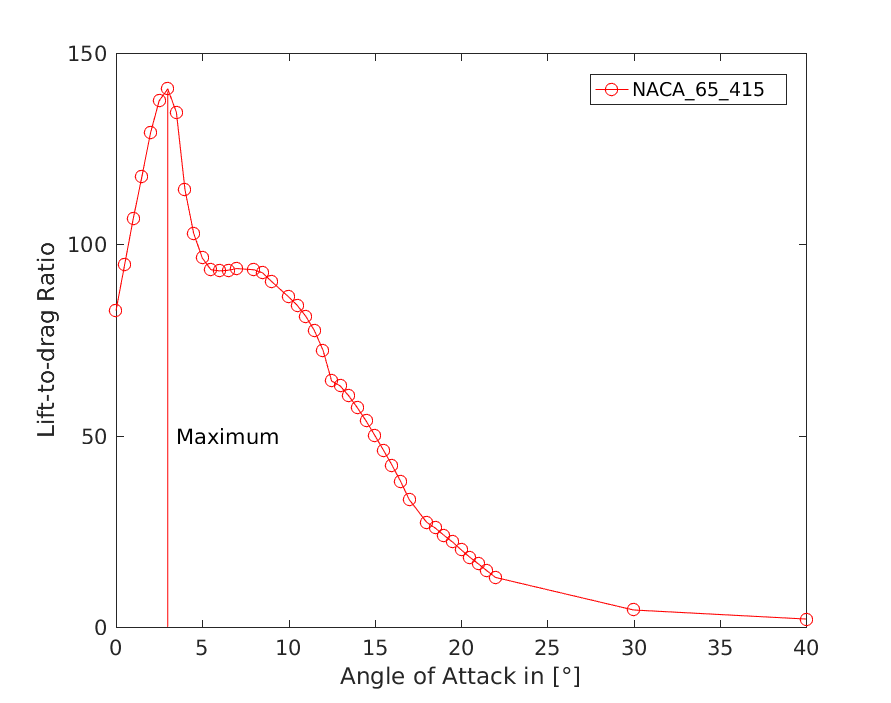
\includegraphics[width=1\linewidth]{../CIP_1/lift_to_drag_ratio_415.png}
  \caption{Lift-to-drag ratio for NACA 65-415}
\end{subfigure}
\begin{subfigure}{0.5\textwidth}
  \centering
  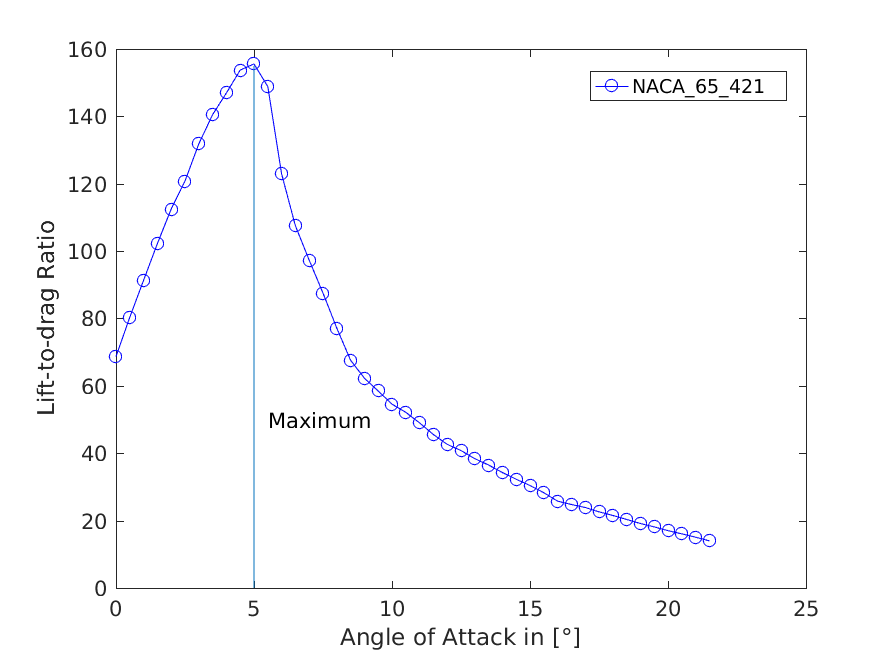
\includegraphics[width=1\linewidth]{../CIP_1/lift_to_drag_ratio_421.png}
  \caption{Lift-to-drag ratio for NACA 65-421}
\end{subfigure}
\caption{Lift-to-drag ratio for different angle of attacks}
\label{fig:comparison_lift_to_drag}
\end{figure}

The figures show that the highest lift-to-drag ratio occurs at low angles of attack. We identified the maximum at 3.0$^\circ$ for NACA 65-415 and 5.0$^\circ$. For higher angles of attack the lift-to-drag ratio shrinks. However in practice there is another method to calculate the optimal design lift coefficient. In the further design we defined the design lift coefficient according to the following equation.
\begin{equation}
c_{l_{design}} = max(cl(max[\frac{c_l}{c_d}], 0.8\cdot c_{l_{max}})
\end{equation}
The results are summarized in the following table:\\
\begin{table}[H]
\begin{tabular}{l | r r r r}
NACA 65-415 & $\alpha$ &$c_l$ &$c_d$ & $c_m$\\
\hline
80\% method& 10 & 1.345 & 0.016 & 0.071\\
lift-to-drag method & 3.0 & 0.710 & 0.005 &  0.088\\
\hline
NACA 65-421 & $\alpha$ &$c_l$ &$c_d$ & $c_m$\\
\hline
80\% method& 11 & 1.255 & 0.026 & 0.055\\
lift-to-drag method & 5.0 & 0.952 & 0.006 &  0.092\\
\end{tabular}
\caption{Main aerodynamic parameters}
\end{table}

As the 80\% method results in a higher lift coefficients for both profiles we selected the corresponding parameters according to the 80\% method.
\newpage
\section{CIP 2}
In the first part of CIP 2 we designed the blade of the wind turbine. In the lecture we discussed two theories which are used to design the blade geometry. Betz and Schmitz theory both have different approaches to calculate the chord length and the twist angle. For the following steps it is import to keep in mind that the given blade consists of 10 blade elements, which are shown in the following figure.
\begin{figure}[H]
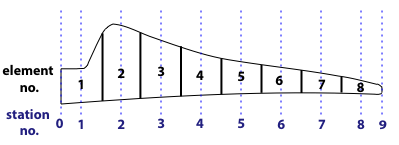
\includegraphics[width=1\linewidth]{../CIP_2/Figures/blade_elements.png}
\caption{Blade Elements}
\label{fig:blade_elemets}
\end{figure}

\subsection{Design your blade according to Betz theory}
Betz theory estimates that the maximum of power that can be extracted from the wind is:
\begin{equation}
P_{betz} = \frac{16}{27}*P_{wind}
\end{equation}
To understand why there is a certain limit, consider that if all energy coming from the wind movement through the turbine the speed afterwards would drop to zero and no new wind could get in.
The principle of Betz's law is derived from the principles of conservation of mass and momentum of the air stream following through and idealized 'actuator disk' (see figure~%\ref{fig:betz_tube}).
%\begin{figure}[H]
%\includegraphics[width=1\linewidth]{figures/betz_tube.png}
%\caption{disk-shaped actuator}
%\label{fig:betz_tube}
%\end{figure}

If we want to design the blade geometry according to this law, the power from the blade element theory has to equal $P_{Betz}$. This leads to the following equations which have been used for the further calculation.\\

Planform:
\begin{equation}
t(r) = 2\pi R \frac{1}{N}\frac{1}{\lambda_a\sqrt{(\lambda_a\frac{r}{R})^2+\frac{4}{9}}}
\end{equation}

Twist angle:
\begin{equation}
\alpha(r) = \arctan(\frac{2}{3}\frac{R}{r\lambda_a)}
\end{equation}
\begin{equation}
\alpha_{twist} = \alpha(r) - \alpha_a
\end{equation}
Using the parameters from CIP 1, we calculated the chord length and the twist angle for each blade segment. And overview is shown in table~\ref{blade_design_betz}.
\begin{table}[H]
\begin{tabular}{c| l l l l l l l l l}
\hline
Station number & 	1&	2&	3	&4	&5	&6	&7	&8	&9\\
\hline
Dist.(rotor center)	m&	4.547&	11.141&	17.734&	24.328&	30.922&	37.516&	44.109&	50.703&	54.000\\
Dist.(blade root)	m&	3.297&	9.891&	16.484&	23.078&	29.672&	36.266&	42.859&	49.453&	52.750\\
\hline
NACA 65-415\\
\hline
Chord length	m&		10.963&	5.989&	3.957&	2.932	&2.324&	1.923&	1.639&	1.428&	1.342\\
Twist angle	deg	&	36.725	&13.436&	5.233&	1.228&	-1.123&	-2.665&	-3.752	&-4.559&	-4.890\\
\hline
NACA 65-421\\
\hline
Chord length	m	&	11.749&	6.418	&4.240&	3.142&	2.490&	2.061	&1.757&	1.531&	1.438
\\
Twist angle	deg	&	35.725&	12.436&	4.233&	0.228	&-2.123&	-3.665	&-4.752&	-5.559	&-5.890\\
\hline
\end{tabular}
\caption{Blade design according to Betz theory}
\label{blade_design_betz}
\end{table}
\subsection{Design according to Schmitz}
The blade design according to Schmitz uses the following equations:\\
Planform:
\begin{equation}
t(r) = \frac{16\pi r}{N c_l}\sin^2(\frac{1}{3}\alpha_1)
\end{equation}

Twist angle:
\begin{equation}
\alpha(r) = \frac{2}{3}\alpha_1
\end{equation}
\begin{equation}
\alpha_{twist} = \alpha(r) - \alpha_a
\end{equation}

where
\begin{equation}
\alpha_1 = \arctan(\frac{R}{\lambda_a rb})
\end{equation}

Using the same approach of the previous section we end up with the following results, shown in table~\ref{blade_design_schmitz}.
\begin{table}[H]
\begin{tabular}{c| l l l l l l l l l}
\hline
Station number & 	1&	2&	3	&4	&5	&6	&7	&8	&9\\
\hline
Dist.(rotor center)	m&	4.547&	11.141&	17.734&	24.328&	30.922&	37.516&	44.109&	50.703&	54.000\\
Dist.(blade root)	m&	3.297&	9.891&	16.484&	23.078&	29.672&	36.266&	42.859&	49.453&	52.750\\
\hline
NACA 65-415\\
\hline
Chord length	m&		6.184 & 5.063 &	3.671&	2.812 & 2.262 & 1.887 & 1.616 &	1.412&	1.328\\
Twist angle	deg	&	28.589	& 12.022 &	4.812 &	1.054 &	-1.210 &	-2.714 &	-3.783	& -4.579 &	-4.906\\
\hline
NACA 65-421\\
\hline
Chord length	m	&	6.628&	5.426&	3.934&	3.013&	2.424&	2.022	&1.732&	1.514&	1.424\\
Twist angle	deg	&	27.589&	11.022&	3.812&	0.0548	&-2.210&	-3.714&-4.783&	-5.579	&-5.906\\
\hline
\end{tabular}
\caption{Blade design according to Schmitz theory}
\label{blade_design_schmitz}
\end{table}
The final blade is designed according to Schmitz theory by a combination of profile 1 and profile 2. The first station has got a cylindrical shape. For stations 2-5 the thinner profile is used, for stations 6-8 the thicker profile is used.Table~\ref{final_blade_design_schmitz} gives more detail about the design rotor blade.
\begin{table}[H]
\begin{tabular}{c| l l l l l l l l l}
\hline
Station number & 	1&	2&	3	&4	&5	&6	&7	&8	&9\\
&Cylinder&65-421&65-421&65-421&65-421& 65-415& 65-415& 65-415&65-415\\
\hline
Blade	m&	3.297&	9.891&	16.484&	23.078&	29.672&	36.266&	42.859&	49.453&	52.750\\
\hline
Chord length	m&	6,628	&5,426&	3,935	&3,014&	2,425&	1,887&	1,617&	1,413&	1,329\\
Twist angle	deg	&	27,590&	11,022&	3,813&	0,055&	-2,211&	-2,715&	-3,783&	-4,580&	-4,907\\
\hline
\end{tabular}
\caption{Final blade design according to Schmitz}
\label{final_blade_design_schmitz}
\end{table}

\newpage
\section{CIP 3 - Performance Curves}
\subsection{Introduction}
In this section we analysed the designed turbine under different pitch angles and tip-speed ratios. The design process of a wind turbine differs from turbine to turbine. In order to compare wind turbines non dimensional coefficients are used. These do not depend on factors like size or wind conditions. The most common coefficient is the power coefficient $c_p$. Further we used the torque coefficient $c_q$ and the thrust coefficient $c_t$.
These coefficient are defined as:
\begin{align*}
c_p = \frac{P}{0.5 *\rho A v^3}\hspace{0.5cm}c_t =  \frac{T}{0.5\rho A v^2}\hspace{0.5cm}c_q = \frac{Q}{0.5\rho A v^2*R}\\
\end{align*}
where:\\
$c_p$ = Power coefficient\\
$c_t$ = Thrust coefficient\\
$c_q$ = Torque coefficient\\
$p$   = Power\\
$\rho$ = Density\\
$A$    = Area\\
$v$	   = Windspeed\\
$R$		= Rotorradius

\subsection{WT\_Perf}
To compute the nondimensional parameters a program called WT\_Perf is used. 
WT\_Perf uses blade-element momentum (BEM) theory to predict the performance of wind turbines. \footnote{WT\_Perf\_Users\_guide.pdf}. It also takes different correction algorithms into account, e.g. Prandtl's tip-loss and hub-loss model.
WT\_Perf can be used from the operating system's command prompt. In order to use WT\_Perf  we configured the input file by updating the 'Turbine Data' section and implementing the calculated blade geometry. WT\_Perf also needs the aerodynamic data of the airfoils. We were able to used the provided data here. Last we defined the range of pitch angle and tip-speed ratio according to the tasks of CIP-3. \\
The following code-snippet gives an idea of the input file structure:
\newpage
\begin{lstlisting}
-----  Turbine Data  -----------------------------------------------------------
    3                NumBlade:                  Number of blades.
62.18                RotorRad:                  Rotor radius.
 1.25                HubRad:                    Hub radius. 
 -3.0                PreCone:                   Precone angle, positive downwind.
  5.0                Tilt:                      Shaft tilt.
  0.0                Yaw:                       Yaw error.
  100                HubHt:                     Hub height.
    8                NumSeg:                    Number of blade segments.

  RElm   Twist   Chord  AFfile  PrntElem
 3.808  26.530   6.988	 1	    FALSE
11.424	 9.594   5.407	 1      FALSE
19.040	 2.661   3.832	 1	    FALSE
26.656	-0.866	 2.906	 1	    FALSE
34.272	-1.967   2.171	 2	    FALSE
41.888	-3.354   1.806	 2	    FALSE
49.504	-4.335   1.544	 2	    FALSE
57.120	-5.066   1.348	 2	    FALSE
\end{lstlisting}
\subsection{3.1,3.2}
As already mentioned we configured the input file according to CIP-3. The generated output file contains values for the power coefficient $c_p$, thrust $T$ and torque $Q$.
For task 3.2 we wrote a small python-program which examines the data and plots the results for the three different nondimensional coefficient mentioned in the introduction of CIP-3: $c_p, c_t$ and $c_q$. Since WT\_Perf only writes the power coefficient we had to calculate $c_t$ and $c_q$. Note that the coefficient are functions of $c_t(\lambda), c_q(\lambda)$.
The following figures display the results for $c_p, c_t$ and $c_q$ with a tip-speed ratio $\lambda$ from one to 20 and pitch angles of : 0,5,10,15,20 and 30 degree. The curves are calculated at rated rotor speed (12.59 rpm).

\begin{figure}[H]
\centering
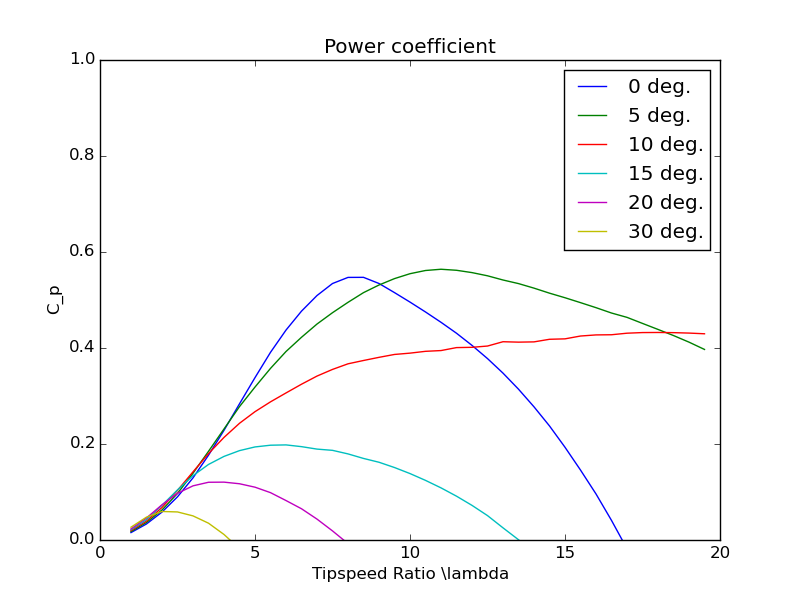
\includegraphics[width=1\linewidth]{../CIP_3/WT_Perf/Output/cp.png}
\caption{Power coefficient}
\label{fig:c-lambda}
\end{figure} 
The $c_p-\lambda$ curve shows different power coefficients at different tip-speeds and pitch-angles. Regarding the maximum for $c_p$ at each curve we identify that they appear at different tip-speed ratios. At pitch angle 5$^\circ$ the maximum $c_p$ is at 0.564 which is very close to the theoretical maximum of 0.592.

\begin{figure}[H]
\centering
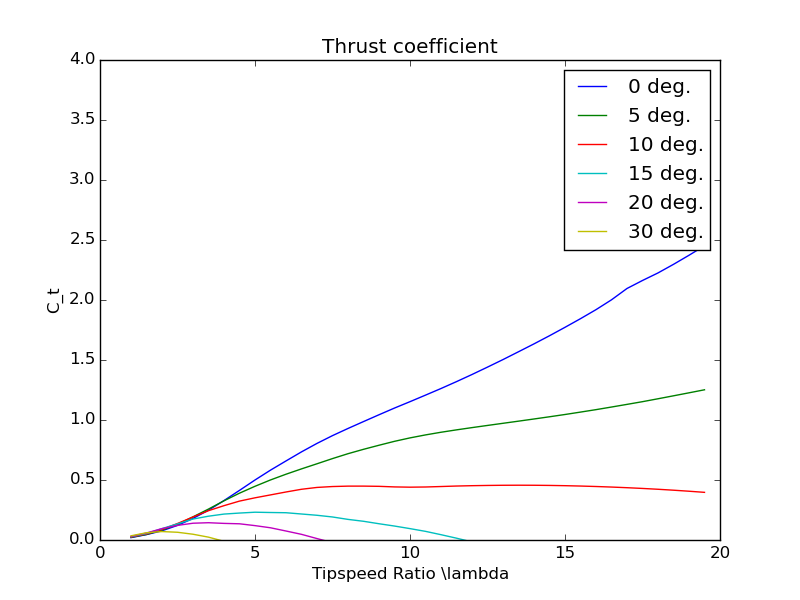
\includegraphics[width=1\linewidth]{../CIP_3/WT_Perf/Output/thrust.png}
\caption{Thrust coefficient}
\label{fig:thrust-coeff}
\end{figure} 
Figure \ref{fig:thrust-coeff} shows the behaviour of the thrust coefficient. 
From 0$^\circ$ to 10$^\circ$ the thrust coefficient reaches high values. For higher pitch angles the resulting thrust coefficient is significantly lower and is equal to zero for higher tip speed ratios. The thrust is directly applied at the tower and can be decreased by increasing the pitch angle.

\begin{figure}[H]
\centering
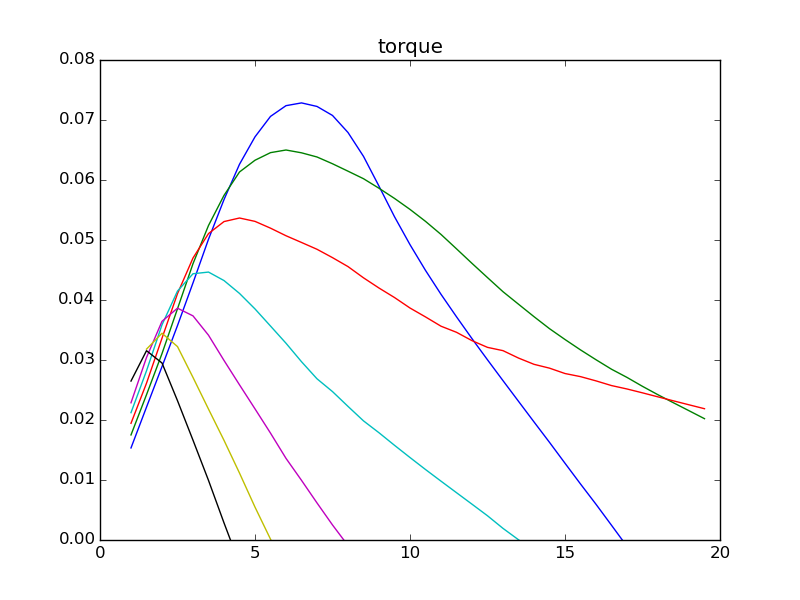
\includegraphics[width=1\linewidth]{../CIP_3/WT_Perf/Output/torque.png}
\caption{Torque coefficient}
\label{fig:torque-coeff}
\end{figure} 
Figure \ref{fig:torque-coeff} shows the torque coefficient for different pitch angles. Compared to the $c_p-\lambda$ the maxima are shifted to the left and decrease with increasing pitch angle.  
\subsection{3.4}
In task 3.4 we were asked to calculate the resulting rotor speed for a rated wind speed of 8 m/s. For the calculation we used our design tip speed ratio:
\begin{align}
\lambda = \frac{\Omega R}{v}\\
n = \frac{60 \lambda v}{2 \pi R} = 10.07 rpm
\end{align}
\subsection{3.5, 3.6}
Again we used WT\_Perf to calculate the resulting operation conditions below rated wind speed. The input parameters are: v = 8 m/s, design top speed ratio $\lambda$ = 8.2 and rotational speed $n$ = 10.07 rpm. The results are shown in the following table:\\

\begin{tabular}{|c |c| c| c| c| c|}
\hline
v & rotor speed & $c_p$ & $c_t$ & $c_q$ & $P$\\
m/s &rpm & - &- &-& kW\\
\hline
8 &10.07&0.544&0.825&0.033& 2054.846\\
\hline
\end{tabular}
Power aus WT\_Perf
\subsection{3.7,3.8}
According to Betz, the wind turbine should be able to extract 7618 kW.
However the rated power of the wind turbine is lower than the power which could be extracted. Therefore pitching is needed. The resulting $c_p$ can be calculated as follows:
\begin{equation}
c_p = \frac{3500000}{0.5 \cdot 1.225 \cdot \pi\cdot  62.18^2 \cdot  12^3} = 0.272
\end{equation}
\subsection{3.9}
\begin{figure}[H]
\centering
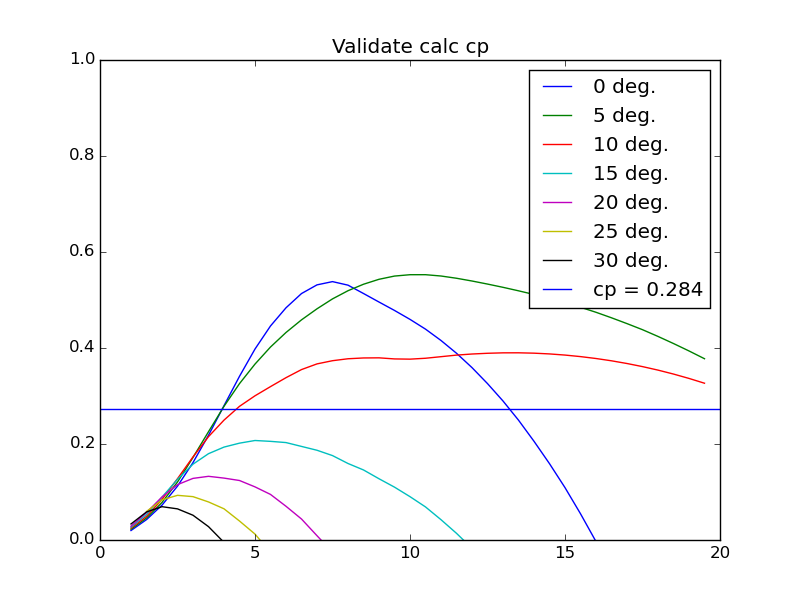
\includegraphics[width=1\linewidth]{../CIP_3/WT_Perf/Output/validated_cp.png}
\caption{Validation of $c_p$}
\label{fig:validate}
The resulting $c_p$ corresponds to a tip speed ratio of 5 with a pitch angle of 10$^\circ$
\end{figure} 
\subsection{3.10}
\begin{align*}
n = \frac{60 \lambda v}{2 \pi R} = 9.21
\end{align*}
\newpage
\section{CIP 4}

The following parameters are relevant for the remainder of this section:

\begin{align*}
	\Omega_{rated} &= 12.59 rpm \text{ (rotor rated speed)} \\
	D &= 5m \text{ (tower diameter)} \\
	E &=211000000000 \frac{N}{m^2} \text{ (elastic modulus)} \\
	l &=100m \text{ (hub height)} \\
	m_{top} &=323000 kg\text{ (nacelle and rotor mass)} \\
	\rho &=7850 \frac{kg}{m^3}\text{ (material density)} \\
\end{align*}

\subsection{Task a}
For tower design resonances of excitation frequencies from the rotating blades must be taken into account. The Eigenfrequency of the tower can thus be obtained by adding a $10 \%$ safety margin to the rotor rated speed which represents the maximum stationary rotor speed:
\begin{equation*}
	f_0 = \Omega_{rated} \cdot 1.1 = \frac{12.59}{60} Hz \cdot 1.1 = 0.23081 Hz
\end{equation*}

\subsection{Task b}
The design range of our turbine is a classical soft-stiff design which results in large wave excitation.

\subsection{Task c}
The wall thickness $t$ can be computed from the following equations:

\begin{align}
f_0 \cot 2 \pi &= \sqrt{\frac{k}{m_{top} + 0.25 m_{tower}}} \\
k &= \frac{3 E \pi D^3 t}{l^3 8} \\
m_{tower} &= \rho \pi D t l\\
\end{align}

By substituting Equations (2) and (3) into (1) we obtain the following equality which can be fed into Matlab in order to solve for the only unknown $t$:\\

\begin{equation*}
0 = \sqrt{\frac{3 E \pi D^3 t}{l^3 8 \cdot (m_{top} + 0.25\rho \pi D t l)}} -f_0 \cdot 2 \pi \\
\end{equation*}

Extract from Matlab code used to solve for variable $t$:\\

\begin{lstlisting}
t=1;
func = @(t) sqrt(3*E*pi*D^3*t/(l^3*8*(mTop+0.25*rho*pi*D+t*l)))-0.23081*2*pi;
t = fsolve(func,t);
\end{lstlisting}

The resulting value for the wall thickness is $t=0.0239m$. The tower mass is then $m_{tower}=295310 kg = 295.31t$. The material cost for this tower would thus be of $147655$ \euro, assuming a price of $500$ \euro /t. Obviously a thicker tower wall leads to a higher price overall (linear increase). As depicted in Figure~\ref{fig:eigfreqWall} a thicker wall leads to a higher Eigenfrequency of the tower as well. However, in this case the relationship is not a linear one due to the exponent of $0.5$ in the formula. Hence, a thicker wall results in a higher Eigenfrequency but the increase is only significant for wall thicknesses up to $0.1m$. Above that the cost increase does not justify the gain in Eigenfrequency.

\begin{figure}[H]
\centering
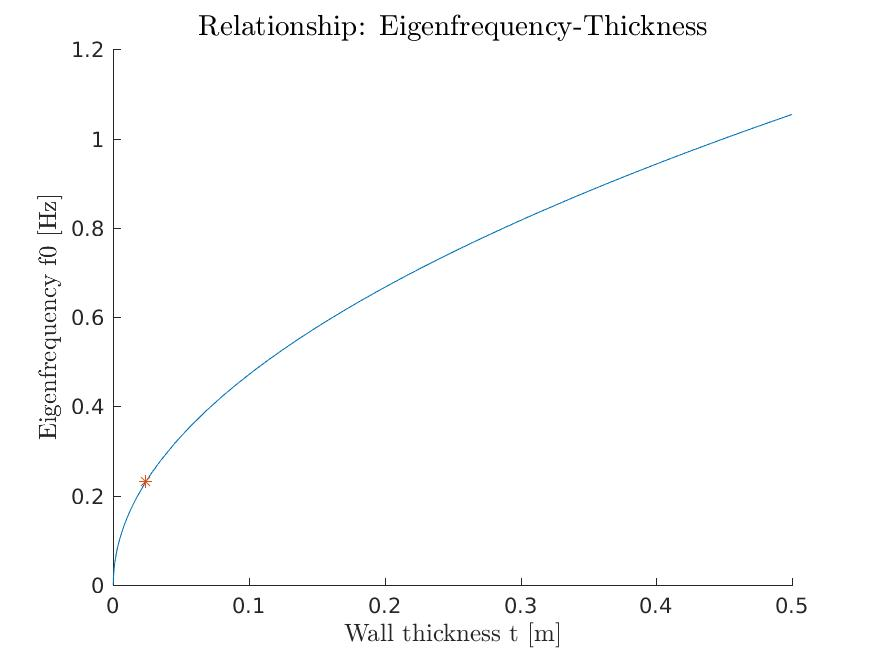
\includegraphics[width=0.6\linewidth]{../CIP_4/figures/eigenfrequency.jpg}
\caption{Effect of wall thickness on Eigenfrequencies}
\label{fig:eigfreqWall}
\end{figure} 

\subsection{Task d}
The Campbell diagram is depicted in Figure~\ref{fig:campbell}  (work in progress)
\begin{figure}[H]
\centering
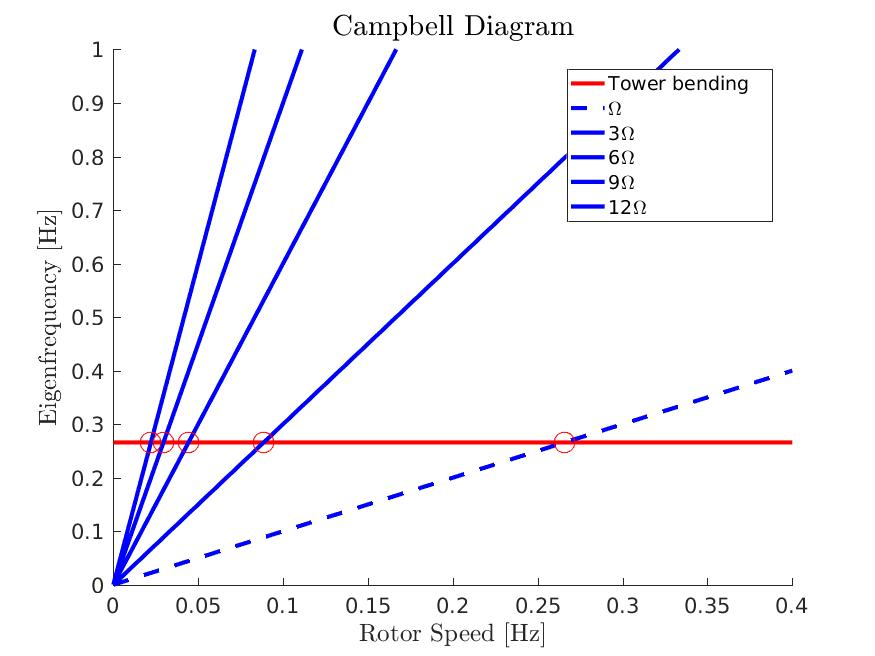
\includegraphics[width=1\linewidth]{../CIP_4/figures/campbell.jpg}
\caption{Campbell Diagram}
\label{fig:campbell}
\end{figure} 
\end{document}
